\newpage
\section{The Quantum Nature of Light}


\subsection{The Photoelectric Effect}
Light of frequency $f$ is directed onto target $T$ and ejects electrons from it. A potential difference $V$ is maintained bewteen target $T$ and collector cup $C$ to sweep up these electrons, said to be \highlight{photoelectrons}. This collection produces a \highlight{photoelectric current $i$} that is measured with meter $A$. 

\begin{figure}[H]
    \centering
    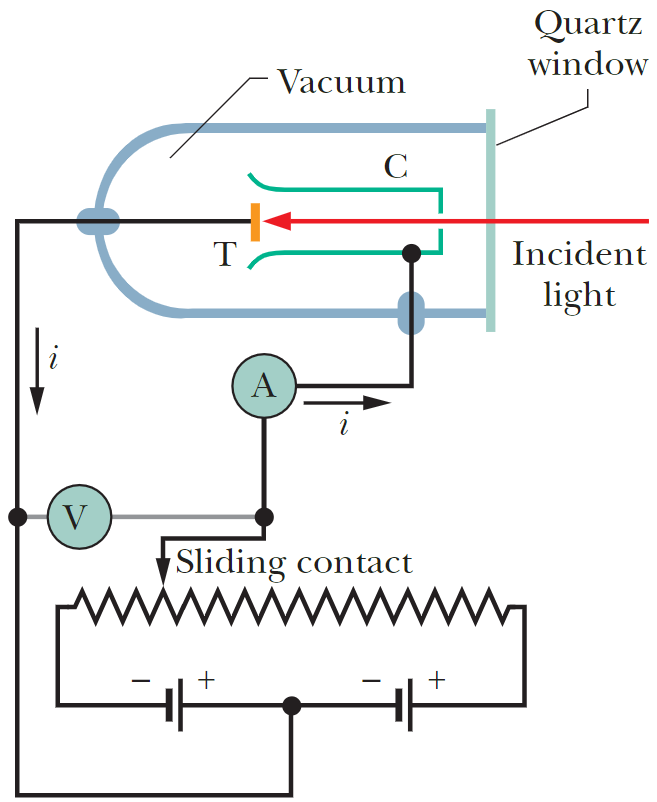
\includegraphics[width=0.209\textwidth]{Lec21/The Photoelectric Effect}
    \caption{The Photoelectric Effect}
\end{figure}

Experiments show that if you direct a beam of light of short enough wavelength onto a clean metal surface, the light will eject the electrons from the surface. We adjust the potential difference $V$ by moving the sliding contact so collector $C$ is slightly negative with respect to target $T$. At the stopping potential $V=V_{stop}$, the readin of meter $A$ has just dropped to zero, the most energetic ejected electrons are turned back just before reaching the collector. Then $K_{max}$, the kinetic energy of these most energetic electrons, is $k_{max}=eV_{stop}$. 

Einstein proposed that electromagnetic radiation or simply light is quantized and exists in elementary amounts (quanta) that we now call \highlight{photons}. According to his proposal, the quantum of a light wave of frequency $f$ has the energy
\begin{align*}
    E=hf=\hbar \omega
\end{align*}
where $h=2\pi \hbar=6.63\times 10^{-34} J\cdot s$ is the \highlight{Planck constant}, and $\omega$ is the angular frequency. The total energy of a light wave of frequency $f$ must be an integer multiple of $hf$, with the smallest amount being $hf$, the energy of a single photon.  

\subsection{Photon, the Quantum of Light}

Einstein further proposed that when light is absorbed or emitted by an object (matter), the absorption or emission event occurs in the atoms of the object. In the absorption event, the energy hf of one photon is transferred from the light to the atom; the photon vanishes and the atom is said to absorb it. For an object consisting of many atoms, there can be many photon absorptions (such as with sunglasses) or photon emissions (such as with lamps). In classical physics, such events involve so much light that we had no need of quantum physics.

The electrons within the target are held by electric forces. To just escape from the target, an electron must pick up a certain minimum energy $W$, where $W$ is a property of the target material called its \highlight{work function}. The energy that can be transferred from the incident light to an electron in the target is that of a single photon $hf$. According the conservation of energy, the kinetic energy $K$ acquired by the electron satisfies
\begin{align*}
    hf=K+W
\end{align*}

In the most favorable circumstance, the electron can escape through the surface without losing any of this kinetic energy in the process, i.e. $K_{max}=hf-W$. Increasing the light intensity increases the number of photons in the light, not the photon energy, so the energy transferred to the kinetic energy of an electron is also unchanged. If the energy $hf$ transferred to an electron by a photon exceeds the work function of the material (if $hf>W$), the electron can esacpe the target. If the energy transferred doesn't exceed the work function (if $hf<W$), the electron can't escape. 

\subsection{Photon Momentum and Compton Scattering}
\subsubsection{Photons Have Momentum}
A photon, or a light quantum, is a particle with energy $E=hf$. It has a velocity of the speed of light $c$, but no mass ($m=0$). Einstein proposed that a quantum of light has linear momentum. According to the theory of relativity

\quad

\begin{align*}
    m=&\frac{m_0}{\sqrt{1-\frac{v^2}{c^2}}}\\
    E=&mc^2=\frac{m_0c^2}{\sqrt{1-\frac{v^2}{c^2}}}\\
    p=&mv=\frac{m_0v}{\sqrt{1-\frac{v^2}{c^2}}}\\
    \therefore \, p=&E\frac{v}{c^2}\\
    \therefore \, E^2=&\frac{m_0^2 c^4}{1-\frac{p^2c^2}{E^2}}\\
    \therefore \, E^2-p^2 c^2=&m_0^2c^4
\end{align*}

\begin{align*}
    \text{Let } E^2-p^2c^2=m_0^2c^4=0
\end{align*}
so the magnitude of the photon momentum is 
\begin{align*}
    p=&\frac{E}{c}=\frac{hf}{c}\\
    =&\frac{h}{\lambda}\\
    =&\hbar k
\end{align*}

\subsubsection{Compton Scattering}
When a photon interacts with matter, energy and momentum are transferred, as if there were a collision bewteen the photon and matter in the classical sense. To demonstrate, Compton measured the wavelength and intensities of a beam of X rays that were scattered in various directions from a carbon target. 

\begin{figure}[H]
    \centering
    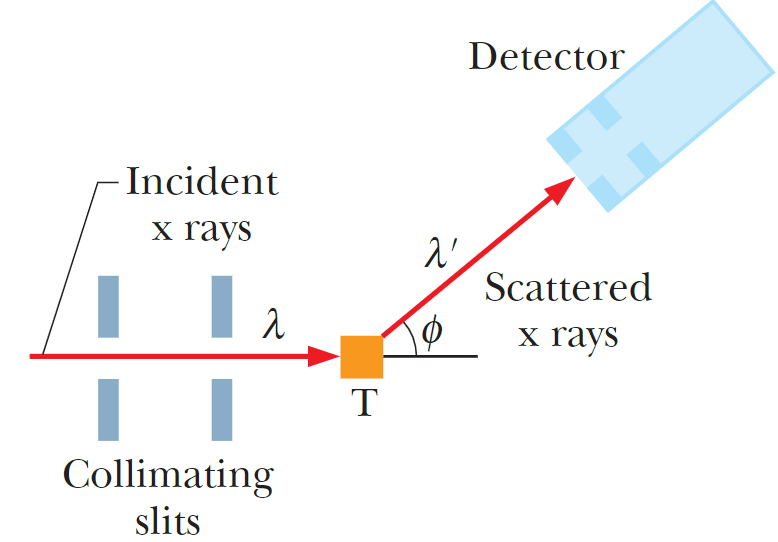
\includegraphics[width=0.309\textwidth]{Lec21/Compton Scattering}
    \caption{Compton Scattering}
\end{figure}

Compton found that although there is only a single wavelength $(\lambda=71.1 pm)$ in the incident X-ray beam, the scattered X rays contain a range of wavelength with two prominent intensity peaks. One peak is centered about the incident wavelength $\lambda$. The other is centered about a wavelength $\lambda^{\prime}$ that is longer than $\lambda$ by an amount $\Delta \lambda$, the \highlight{Compton shift}. The value of the Compton shift varies with the angle at which the scattered X rays are detected and is greater for a greater angle. 

\begin{figure}[H]
    \centering
    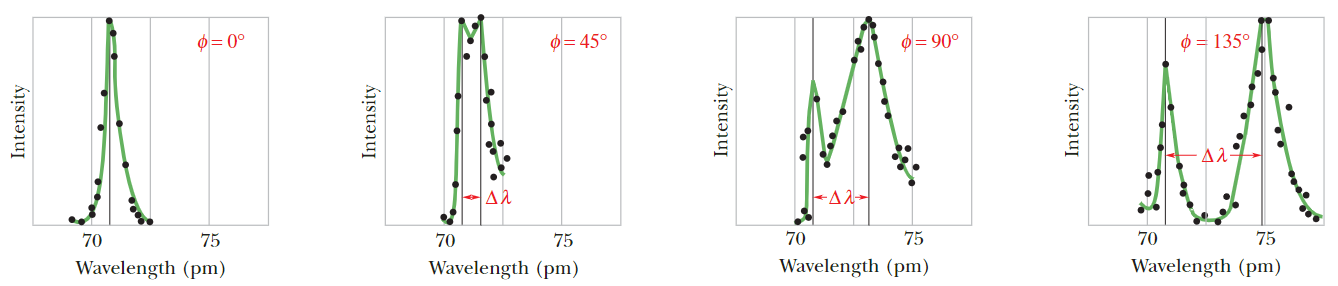
\includegraphics[width=0.309\textwidth]{Lec21/X-ray}
    \caption{X-ray}
\end{figure}

In classical physics, an electron in the carbon target undergoes forced oscillations in the sinusoidally oscillating electromagnetic wave. Hence, the electron should send out scattered waves at the \highlight{same frequency}. 

\begin{figure}[H]
    \centering
    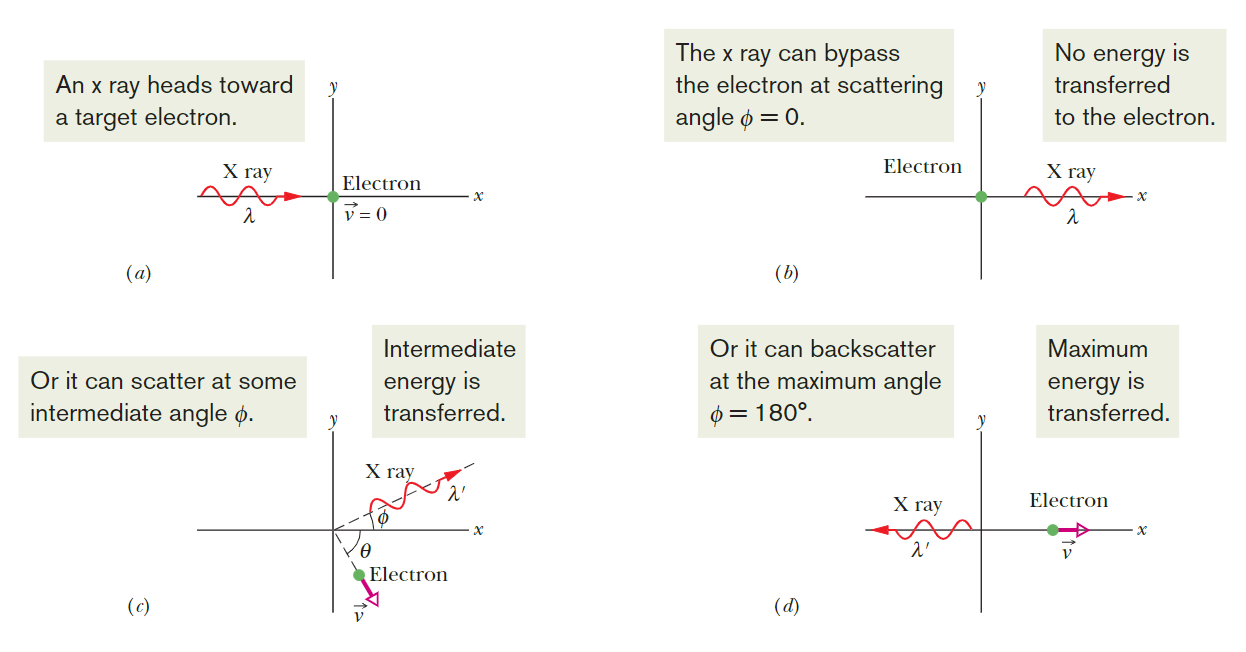
\includegraphics[width=0.479\textwidth]{Lec21/With quantum physics and relativity}
    \caption{With quantum physics and relativity}
\end{figure}


With quantum physics and relativity, the energy and momentum conservation becomes
\begin{align*}
    \text{Energy: }&\frac{hc}{\lambda}+mc^2=\frac{hc}{\lambda^{\prime}}+\gamma mc^2\\
    \text{Momentum: }&\left\{\begin{array}{cc}
         \frac{h}{\lambda} = \frac{h}{\lambda^{\prime}}\cos\phi +\gamma mv \cos\theta & \text{in x}\\
         0=\frac{h}{\lambda^{\prime}}\sin\phi +\gamma mv \sin\theta & \text{in y}
    \end{array}\right.
\end{align*}

To solve for $\Delta \lambda$, we rearrange the equations into
\begin{align*}
    \frac{h}{\lambda}-\frac{h}{\lambda^{\prime}}+mc=&\gamma mc\\
    \frac{h}{\lambda}-\frac{h}{\lambda^{\prime}}\cos\phi=&\gamma  mv\cos\theta\\
    \frac{h}{\lambda^{\prime}}\sin\phi=&\gamma mv\sin\theta
\end{align*}

Take the square of the first equation, subtracting the squares of the ohter two, we find, after some algebra
\begin{align*}
    \Delta\lambda=&\frac{h}{mc}(1-\cos\phi)\\
    =&\frac{2h}{mc}\sin^2\frac{\phi}{2}
\end{align*}

The quantity $\frac{h}{mc}$ is a constant called the \highlight{Compton wavelength}. Its value depends on the mass $m$ of the particle from which the X rays scatter. Strictly speaking, the particle can be a loosely bound
electron, or a carbon atom (with tightly bound electrons). 
\begin{itemize}
    \item For an electron, the Compton wavelength is 
    \begin{align*}
        \frac{h}{mc}=\frac{hc}{mc^2}=\frac{12400\, eV\cdot \text{\AA} }{511,00\,  eV}=2.426 \, pm
    \end{align*} 
    \item For a carbon atom, the Compton wavelength is $12\times 1836\approx 22,000$ tiems samlled and, hence, can be neglected. Therefore, there is a peak at the incident wavelength at any angle.
\end{itemize}

\subsection{Angular Momentum of Photons and Polarization}

According to the quantum-mechanical description, a photon also has an intrinsic spin angular momentum, which is either $-\hbar$ or $+\hbar$, where the signs indicate right- or left-handedness, respectively. Whenever a charged particle emits or absorbs electromagnetic radiation, along with changes in its energy and linear momentum, it will undergo a change of $\pm\hbar$ in its angular momentum. The energy transferred to a target by an incident monocromatic electromagnetic wave can be envisaged as being transported in the form of a stream of identical photons. A purely left-circularly (right-circularly) polarized plane wave will impart angular momentum to the target as if all the constituent photons in the bem had their spins aligned in (opposite) the direction of propagation. 

\begin{figure}[H]
    \centering
    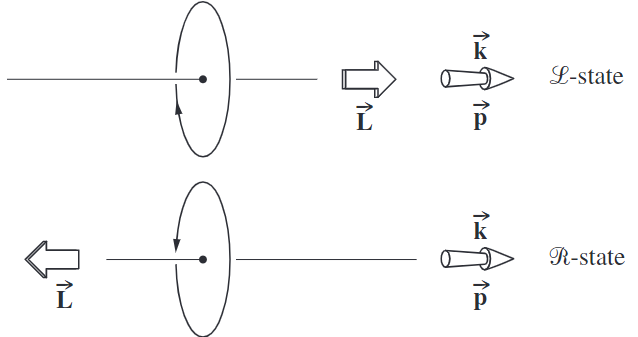
\includegraphics[width=0.309\textwidth]{Lec21/Angular Momentum of Photons}
    \caption{Angular Momentum of Photons}
\end{figure}

A beam of linearly polarized light will interact with matter as if it were composed, at that instant, of equal numbers of right- and left-handed photons. There is a subtle point. \highlight{Strictly speaking, we can't say that th beam is actually made up of precisely equal amounts of well-defined right- and left-handed photons; the photons are all identical. Rather, each individual photon exists in either spin state with equal likelihood}. 
\begin{align*}
    \ket{H}=\frac{\ket{R}+\ket{L}}{\sqrt{2}}=\frac{1}{\sqrt{2}}\left[\frac{1}{\sqrt{2}}\begin{pmatrix}
        1\\-i
    \end{pmatrix}+\frac{1}{\sqrt{2}}\begin{pmatrix}
        1\\i
    \end{pmatrix}  \right]
\end{align*}
This probabilistic interpretation also applies to diagonally polarized light
\begin{align*}
    \ket{D}=&\frac{1}{\sqrt{2}}\begin{pmatrix}
        1\\1
    \end{pmatrix}=\frac{\ket{H}+\ket{V}}{\sqrt{2}}\\
    \ket{A}=&\frac{1}{\sqrt{2}}\begin{pmatrix}
        1\\-1
    \end{pmatrix}=\frac{\ket{H}-\ket{V}}{\sqrt{2}}
\end{align*}
Or inversely,
\begin{align*}
    \ket{H}=&\frac{\ket{D}+\ket{A}}{\sqrt{2}}\\
    \ket{V}=&\frac{\ket{D}-\ket{A}}{\sqrt{2}}
\end{align*}
